\documentclass[11pt, letterpaper]{article}

% Fonts and Encoding
\usepackage[utf8]{inputenc}
\usepackage[T1]{fontenc}
\usepackage{lmodern} % High-quality Latin Modern vector font

% Math and Symbols
\usepackage{amsmath, amssymb, amsthm, amsfonts, mathrsfs, mathtools}

% Layout and Geometry
\usepackage{geometry}
\geometry{letterpaper, margin=1in}
\setlength{\parindent}{0pt}
\setlength{\parskip}{0.6em}

% Formatting and Graphics
\usepackage{graphicx, xcolor, enumitem, booktabs, array, tabularx}

% TikZ for Illustrations
\usepackage{tikz}
\usetikzlibrary{arrows.meta, positioning, shapes.geometric, calc, backgrounds, matrix}

% Clickable Links and TOC
\usepackage{hyperref}
\hypersetup{
    colorlinks=true,
    linkcolor=blue,
    filecolor=magenta,      
    urlcolor=cyan,
    pdftitle={Advanced Mathematics Topic},
}

% Theorem Environments
\newtheorem{theorem}{Theorem}[section]
\newtheorem{lemma}[theorem]{Lemma}
\newtheorem{proposition}[theorem]{Proposition}
\newtheorem{corollary}[theorem]{Corollary}
\theoremstyle{definition}
\newtheorem{definition}{Definition}[section]
\newtheorem{axiom}{Axiom}[section]
\newtheorem{example}{Example}[section]
\theoremstyle{remark}
\newtheorem{remark}{Remark}[section]

% Custom Commands (Enforced standard notation)
\newcommand{\R}{\mathbb{R}}
\newcommand{\N}{\mathbb{N}}
\newcommand{\Z}{\mathbb{Z}}
\newcommand{\Q}{\mathbb{Q}}
\newcommand{\E}{\mathbb{E}}
\newcommand{\Prob}{\mathbb{P}}
\newcommand{\F}{\mathcal{F}}

\begin{document}

\title{\textbf{Mastering Convolution and the Dirac Delta Function}}
\author{Tashfeen Omran}
\date{\today}
\maketitle

\tableofcontents
\newpage

\section{Part 1: Comprehensive Introduction, Context, and Prerequisites}

\subsection{Core Concepts}
In the study of linear differential equations and systems analysis, we frequently encounter situations where the output of a system depends not just on the instantaneous input, but on the accumulated history of past inputs. The mathematical operation that captures this "blending" of past and present is called \textbf{Convolution}. 

Given two piecewise continuous functions $f(t)$ and $g(t)$ defined on $[0, \infty)$, their convolution, denoted as $(f * g)(t)$, is defined by the integral:
\[
(f * g)(t) = \int_0^t f(t - v)g(v) \, dv
\]
This operation takes two functions and produces a third. It is commutative ($f * g = g * f$), associative, and distributes over addition. 

The \textbf{Dirac Delta Function}, $\delta(t)$, is a generalized function (or distribution) used to model phenomena like instantaneous impulses (e.g., a hammer strike). It is characterized by being zero everywhere except at $t=0$, where it is "infinite," such that its total integral over $\R$ is $1$. Its defining sifting property is $\int_{-\infty}^{\infty} f(t)\delta(t-a) \, dt = f(a)$.

\subsection{Intuition and Derivation}
Imagine a system that receives an input signal $g(v)$ at time $v$. The system's response to a unit impulse decays or evolves over time according to a function $f(t)$. At a later time $t$, the residual effect of the input from time $v$ is proportional to $f(t-v)$. To find the total response at time $t$, we must sum (integrate) the residual effects of all past inputs from $v=0$ to $v=t$. This naturally yields the convolution integral.

The \textbf{Convolution Theorem} bridges the time domain and the frequency (Laplace) domain. It states that the Laplace transform of a convolution of two functions is simply the algebraic product of their individual Laplace transforms:
\[
\mathscr{L}\{f * g\}(s) = F(s)G(s)
\]
This is derived by writing the definition of the Laplace transform of the convolution integral, reversing the order of integration (using the unit step function to manage bounds), and factoring the resulting double integral into two independent Laplace transforms.

\subsection{Historical Context and Motivation}
In the early 20th century, mathematicians like Vito Volterra studied integro-differential equations to model population dynamics with "hereditary influences" (where the current rate of change depends on the history of the population). Simultaneously, Oliver Heaviside and Paul Dirac were developing operational calculus to solve electrical engineering problems involving sudden surges of current. The convolution theorem provided a rigorous, unified framework to solve these complex equations algebraically in the Laplace domain before transforming them back to the time domain.

\subsection{Key Formulas}
\begin{itemize}
    \item \textbf{Convolution Integral:} $(f * g)(t) = \int_0^t f(t - v)g(v) \, dv$
    \item \textbf{Convolution Theorem:} $\mathscr{L}^{-1}\{F(s)G(s)\} = (f * g)(t)$
    \item \textbf{Transfer Function:} $H(s) = \frac{Y(s)}{G(s)} = \frac{1}{as^2 + bs + c}$
    \item \textbf{Impulse Response:} $h(t) = \mathscr{L}^{-1}\{H(s)\}$
    \item \textbf{General IVP Solution:} $y(t) = (h * g)(t) + y_k(t)$ (where $y_k$ solves the homogeneous IVP)
    \item \textbf{Dirac Sifting Property:} $\int_{-\infty}^{\infty} f(t)\delta(t-a) \, dt = f(a)$
\end{itemize}

\subsection{Prerequisites}
To master this topic, you must be proficient in:
1. \textbf{Laplace Transforms:} Forward and inverse transforms of standard functions ($e^{at}$, $\sin(kt)$, $t^n$).
2. \textbf{Partial Fraction Decomposition:} Breaking down complex rational functions in the $s$-domain.
3. \textbf{Integration Techniques:} Integration by parts, $u$-substitution, and trigonometric identities (especially product-to-sum formulas).
4. \textbf{Completing the Square:} Essential for finding inverse Laplace transforms of irreducible quadratic denominators.

\newpage
\section{Part 2: Detailed Homework Solutions}

\textbf{Problem 1:} Use the convolution theorem to obtain a formula for the solution to $y'' - 2y' + y = g(t); \quad y(0) = -1, \quad y'(0) = 1$.
\textit{Solution:}
Take the Laplace transform of both sides:
\begin{align*}
[s^2Y(s) - sy(0) - y'(0)] - 2[sY(s) - y(0)] + Y(s) &= G(s) \\[4pt]
s^2Y(s) + s - 1 - 2sY(s) - 2 + Y(s) &= G(s) \\[4pt]
(s^2 - 2s + 1)Y(s) + s - 3 &= G(s) \\[4pt]
(s-1)^2Y(s) &= G(s) - s + 3 \\[4pt]
Y(s) &= \frac{G(s)}{(s-1)^2} - \frac{s-3}{(s-1)^2}
\end{align*}
We decompose the second term: $\frac{s-3}{(s-1)^2} = \frac{s-1-2}{(s-1)^2} = \frac{1}{s-1} - \frac{2}{(s-1)^2}$.
\begin{align*}
Y(s) &= \frac{G(s)}{(s-1)^2} - \frac{1}{s-1} + \frac{2}{(s-1)^2}
\end{align*}
Taking the inverse Laplace transform, noting $\mathscr{L}^{-1}\left\{\frac{1}{(s-1)^2}\right\} = t e^t$:
\begin{align*}
y(t) &= (t e^t) * g(t) - e^t + 2t e^t \\[4pt]
y(t) &= \int_0^t (t-v)e^{t-v}g(v) \, dv - e^t + 2t e^t
\end{align*}

\textbf{Problem 2:} $y'' + 9y = g(t); \quad y(0) = 1, \quad y'(0) = 0$.
\textit{Solution:}
\begin{align*}
[s^2Y(s) - s(1) - 0] + 9Y(s) &= G(s) \\[4pt]
(s^2 + 9)Y(s) &= G(s) + s \\[4pt]
Y(s) &= \frac{G(s)}{s^2+9} + \frac{s}{s^2+9}
\end{align*}
Taking the inverse Laplace transform:
\begin{align*}
y(t) &= \left(\frac{1}{3}\sin(3t)\right) * g(t) + \cos(3t) \\[4pt]
y(t) &= \frac{1}{3}\int_0^t \sin(3(t-v))g(v) \, dv + \cos(3t)
\end{align*}

\textbf{Problem 3:} $y'' + 4y' + 5y = g(t); \quad y(0) = 1, \quad y'(0) = 1$.
\textit{Solution:}
\begin{align*}
[s^2Y(s) - s - 1] + 4[sY(s) - 1] + 5Y(s) &= G(s) \\[4pt]
(s^2 + 4s + 5)Y(s) - s - 5 &= G(s) \\[4pt]
Y(s) &= \frac{G(s)}{s^2+4s+5} + \frac{s+5}{s^2+4s+5}
\end{align*}
Complete the square for the denominator: $s^2+4s+5 = (s+2)^2 + 1$.
\begin{align*}
Y(s) &= \frac{G(s)}{(s+2)^2+1} + \frac{s+2}{(s+2)^2+1} + \frac{3}{(s+2)^2+1}
\end{align*}
Taking the inverse Laplace transform:
\begin{align*}
y(t) &= (e^{-2t}\sin t) * g(t) + e^{-2t}\cos t + 3e^{-2t}\sin t \\[4pt]
y(t) &= \int_0^t e^{-2(t-v)}\sin(t-v)g(v) \, dv + e^{-2t}(\cos t + 3\sin t)
\end{align*}

\textbf{Problem 4:} $y'' + y = g(t); \quad y(0) = 0, \quad y'(0) = 1$.
\textit{Solution:}
\begin{align*}
[s^2Y(s) - 1] + Y(s) &= G(s) \\[4pt]
(s^2 + 1)Y(s) &= G(s) + 1 \\[4pt]
Y(s) &= \frac{G(s)}{s^2+1} + \frac{1}{s^2+1}
\end{align*}
Taking the inverse Laplace transform:
\begin{align*}
y(t) &= \sin t * g(t) + \sin t = \int_0^t \sin(t-v)g(v) \, dv + \sin t
\end{align*}

\textbf{Problem 5:} Find the inverse Laplace transform of $\frac{1}{s(s^2+1)}$.
\textit{Solution:}
Let $F(s) = \frac{1}{s}$ and $G(s) = \frac{1}{s^2+1}$. Then $f(t) = 1$ and $g(t) = \sin t$.
\begin{align*}
\mathscr{L}^{-1}\left\{\frac{1}{s(s^2+1)}\right\} &= 1 * \sin t = \int_0^t 1 \cdot \sin(v) \, dv \\[4pt]
&= \left[ -\cos v \right]_0^t = -\cos t - (-\cos 0) = 1 - \cos t
\end{align*}

\textbf{Problem 6:} Find the inverse Laplace transform of $\frac{1}{(s+1)(s+2)}$.
\textit{Solution:}
Let $F(s) = \frac{1}{s+1}$ and $G(s) = \frac{1}{s+2}$. Then $f(t) = e^{-t}$ and $g(t) = e^{-2t}$.
\begin{align*}
\mathscr{L}^{-1}\left\{\frac{1}{(s+1)(s+2)}\right\} &= e^{-t} * e^{-2t} = \int_0^t e^{-(t-v)}e^{-2v} \, dv \\[4pt]
&= e^{-t} \int_0^t e^{-v} \, dv = e^{-t} \left[ -e^{-v} \right]_0^t \\[4pt]
&= e^{-t}(1 - e^{-t}) = e^{-t} - e^{-2t}
\end{align*}

\textbf{Problem 7:} Find the inverse Laplace transform of $\frac{14}{(s+2)(s-5)}$.
\textit{Solution:}
Let $F(s) = \frac{1}{s+2}$ and $G(s) = \frac{14}{s-5}$. Then $f(t) = e^{-2t}$ and $g(t) = 14e^{5t}$.
\begin{align*}
\mathscr{L}^{-1}\left\{\frac{14}{(s+2)(s-5)}\right\} &= \int_0^t e^{-2(t-v)} 14e^{5v} \, dv = 14e^{-2t} \int_0^t e^{7v} \, dv \\[4pt]
&= 14e^{-2t} \left[ \frac{e^{7v}}{7} \right]_0^t = 2e^{-2t}(e^{7t} - 1) = 2e^{5t} - 2e^{-2t}
\end{align*}

\textbf{Problem 8:} Find the inverse Laplace transform of $\frac{1}{(s^2+4)^2}$.
\textit{Solution:}
Let $F(s) = G(s) = \frac{1}{s^2+4}$. Then $f(t) = g(t) = \frac{1}{2}\sin(2t)$.
\begin{align*}
\mathscr{L}^{-1}\left\{\frac{1}{(s^2+4)^2}\right\} &= \frac{1}{2}\sin(2t) * \frac{1}{2}\sin(2t) = \frac{1}{4} \int_0^t \sin(2t-2v)\sin(2v) \, dv
\end{align*}
Using the identity $\sin A \sin B = \frac{1}{2}[\cos(A-B) - \cos(A+B)]$:
\begin{align*}
&= \frac{1}{8} \int_0^t [\cos(2t-4v) - \cos(2t)] \, dv \\[4pt]
&= \frac{1}{8} \left[ \frac{\sin(2t-4v)}{-4} - v\cos(2t) \right]_0^t \\[4pt]
&= \frac{1}{8} \left( \frac{\sin(-2t)}{-4} - t\cos(2t) - \frac{\sin(2t)}{-4} \right) \\[4pt]
&= \frac{1}{8} \left( \frac{\sin(2t)}{2} - t\cos(2t) \right) = \frac{\sin(2t) - 2t\cos(2t)}{16}
\end{align*}

\textbf{Problem 9:} Find the inverse Laplace transform of $\frac{s}{(s^2+1)^2}$.
\textit{Solution:}
Let $F(s) = \frac{s}{s^2+1}$ and $G(s) = \frac{1}{s^2+1}$. Then $f(t) = \cos t$ and $g(t) = \sin t$.
\begin{align*}
\mathscr{L}^{-1}\left\{\frac{s}{(s^2+1)^2}\right\} &= \cos t * \sin t = \int_0^t \cos(t-v)\sin(v) \, dv
\end{align*}
Using $\cos A \sin B = \frac{1}{2}[\sin(A+B) - \sin(A-B)]$:
\begin{align*}
&= \frac{1}{2} \int_0^t [\sin(t) - \sin(t-2v)] \, dv \\[4pt]
&= \frac{1}{2} \left[ v\sin t - \frac{\cos(t-2v)}{2} \right]_0^t \\[4pt]
&= \frac{1}{2} \left( t\sin t - \frac{\cos(-t)}{2} + \frac{\cos t}{2} \right) = \frac{1}{2}t\sin t
\end{align*}

\textbf{Problem 10:} Find the inverse Laplace transform of $\frac{1}{s^3(s^2+1)}$.
\textit{Solution:}
Let $F(s) = \frac{1}{s^2}$ and $G(s) = \frac{1}{s(s^2+1)}$. From Problem 5, $g(t) = 1 - \cos t$. $f(t) = t$.
\begin{align*}
\mathscr{L}^{-1}\left\{\frac{1}{s^3(s^2+1)}\right\} &= t * (1 - \cos t) = \int_0^t (t-v)(1 - \cos v) \, dv \\[4pt]
&= \int_0^t (t - t\cos v - v + v\cos v) \, dv \\[4pt]
&= \left[ tv - t\sin v - \frac{v^2}{2} + (v\sin v + \cos v) \right]_0^t \\[4pt]
&= \left( t^2 - t\sin t - \frac{t^2}{2} + t\sin t + \cos t \right) - (1) = \frac{t^2}{2} + \cos t - 1
\end{align*}

\textbf{Problem 11:} Find the inverse Laplace transform of $\frac{s}{(s-1)(s+2)}$.
\textit{Solution:}
Using the hint: $\frac{s}{s-1} = 1 + \frac{1}{s-1}$.
\begin{align*}
\frac{s}{(s-1)(s+2)} &= \left(1 + \frac{1}{s-1}\right)\frac{1}{s+2} = \frac{1}{s+2} + \frac{1}{(s-1)(s+2)}
\end{align*}
The inverse transform of the first term is $e^{-2t}$. For the second term, we use convolution:
\begin{align*}
\mathscr{L}^{-1}\left\{\frac{1}{(s-1)(s+2)}\right\} &= e^t * e^{-2t} = \int_0^t e^{t-v}e^{-2v} \, dv = e^t \int_0^t e^{-3v} \, dv \\[4pt]
&= e^t \left[ \frac{e^{-3v}}{-3} \right]_0^t = e^t \left( \frac{e^{-3t} - 1}{-3} \right) = \frac{1}{3}e^t - \frac{1}{3}e^{-2t}
\end{align*}
Adding the first term back: $y(t) = e^{-2t} + \frac{1}{3}e^t - \frac{1}{3}e^{-2t} = \frac{1}{3}e^t + \frac{2}{3}e^{-2t}$.

\textbf{Problem 12:} Find the inverse Laplace transform of $\frac{s+1}{(s^2+1)^2}$.
\textit{Solution:}
Split the fraction: $\frac{s}{(s^2+1)^2} + \frac{1}{(s^2+1)^2}$.
Using the results from Problems 8 and 9 (with $a=1$):
\begin{align*}
y(t) &= \frac{1}{2}t\sin t + \frac{\sin t - t\cos t}{2} = \frac{1}{2}(\sin t + t\sin t - t\cos t)
\end{align*}

\textbf{Problem 13:} Find the Laplace transform of $f(t) = \int_0^t (t-v)e^{3v} \, dv$.
\textit{Solution:}
This is the convolution of $t$ and $e^{3t}$.
\begin{align*}
\mathscr{L}\{t * e^{3t}\} &= \mathscr{L}\{t\} \cdot \mathscr{L}\{e^{3t}\} = \left(\frac{1}{s^2}\right)\left(\frac{1}{s-3}\right) = \frac{1}{s^2(s-3)}
\end{align*}

\textbf{Problem 14:} Find the Laplace transform of $f(t) = \int_0^t e^v \sin(t-v) \, dv$.
\textit{Solution:}
This is the convolution of $\sin t$ and $e^t$.
\begin{align*}
\mathscr{L}\{\sin t * e^t\} &= \mathscr{L}\{\sin t\} \cdot \mathscr{L}\{e^t\} = \left(\frac{1}{s^2+1}\right)\left(\frac{1}{s-1}\right) = \frac{1}{(s^2+1)(s-1)}
\end{align*}

\textbf{Problem 15:} Solve the integral equation $y(t) + 3\int_0^t y(v)\sin(t-v) \, dv = t$.
\textit{Solution:}
Take the Laplace transform:
\begin{align*}
Y(s) + 3Y(s)\left(\frac{1}{s^2+1}\right) &= \frac{1}{s^2} \\[4pt]
Y(s)\left(1 + \frac{3}{s^2+1}\right) &= \frac{1}{s^2} \implies Y(s)\left(\frac{s^2+4}{s^2+1}\right) = \frac{1}{s^2} \\[4pt]
Y(s) &= \frac{s^2+1}{s^2(s^2+4)} = \frac{A}{s} + \frac{B}{s^2} + \frac{Cs+D}{s^2+4}
\end{align*}
By partial fractions, $B = 1/4$, $D = 3/4$, $A=C=0$.
\begin{align*}
Y(s) &= \frac{1/4}{s^2} + \frac{3/4}{s^2+4} \implies y(t) = \frac{1}{4}t + \frac{3}{8}\sin(2t)
\end{align*}

\textbf{Problem 16:} Solve $y(t) + \int_0^t e^{t-v}y(v) \, dv = \sin t$.
\textit{Solution:}
\begin{align*}
Y(s) + Y(s)\left(\frac{1}{s-1}\right) &= \frac{1}{s^2+1} \\[4pt]
Y(s)\left(\frac{s}{s-1}\right) &= \frac{1}{s^2+1} \implies Y(s) = \frac{s-1}{s(s^2+1)} = \frac{s}{s(s^2+1)} - \frac{1}{s(s^2+1)} \\[4pt]
Y(s) &= \frac{1}{s^2+1} - \frac{1}{s(s^2+1)}
\end{align*}
Using Problem 5 for the second term:
\begin{align*}
y(t) &= \sin t - (1 - \cos t) = \sin t + \cos t - 1
\end{align*}

\textbf{Problem 17:} Solve $y(t) + \int_0^t (t-v)y(v) \, dv = 1$.
\textit{Solution:}
\begin{align*}
Y(s) + Y(s)\left(\frac{1}{s^2}\right) &= \frac{1}{s} \implies Y(s)\left(\frac{s^2+1}{s^2}\right) = \frac{1}{s} \\[4pt]
Y(s) &= \frac{s}{s^2+1} \implies y(t) = \cos t
\end{align*}

\textbf{Problem 18:} Solve $y(t) + \int_0^t (t-v)y(v) \, dv = t^2$.
\textit{Solution:}
\begin{align*}
Y(s)\left(\frac{s^2+1}{s^2}\right) &= \frac{2}{s^3} \implies Y(s) = \frac{2}{s(s^2+1)} = 2\left(\frac{1}{s} - \frac{s}{s^2+1}\right) \\[4pt]
y(t) &= 2(1 - \cos t)
\end{align*}

\textbf{Problem 19:} Solve $y(t) + \int_0^t (t-v)^2 y(v) \, dv = t^3 + 3$.
\textit{Solution:}
\begin{align*}
Y(s) + Y(s)\left(\frac{2}{s^3}\right) &= \frac{6}{s^4} + \frac{3}{s} \implies Y(s)\left(\frac{s^3+2}{s^3}\right) = \frac{3s^3+6}{s^4} \\[4pt]
Y(s) &= \frac{3(s^3+2)}{s^4} \cdot \frac{s^3}{s^3+2} = \frac{3}{s} \implies y(t) = 3
\end{align*}

\textbf{Problem 20:} Solve $y'(t) + \int_0^t (t-v)y(v) \, dv = t, \quad y(0)=0$.
\textit{Solution:}
\begin{align*}
sY(s) - 0 + Y(s)\left(\frac{1}{s^2}\right) &= \frac{1}{s^2} \implies Y(s)\left(\frac{s^3+1}{s^2}\right) = \frac{1}{s^2} \\[4pt]
Y(s) &= \frac{1}{s^3+1} = \frac{1}{(s+1)(s^2-s+1)}
\end{align*}
Partial fractions: $\frac{1}{(s+1)(s^2-s+1)} = \frac{1/3}{s+1} + \frac{-1/3 s + 2/3}{s^2-s+1}$.
Complete the square: $s^2-s+1 = (s-1/2)^2 + 3/4$.
\begin{align*}
Y(s) &= \frac{1}{3}\frac{1}{s+1} - \frac{1}{3}\frac{s-1/2}{(s-1/2)^2+3/4} + \frac{1}{3}\frac{1/2}{(s-1/2)^2+3/4} \\[4pt]
y(t) &= \frac{1}{3}e^{-t} - \frac{1}{3}e^{t/2}\cos\left(\frac{\sqrt{3}}{2}t\right) + \frac{1}{3\sqrt{3}}e^{t/2}\sin\left(\frac{\sqrt{3}}{2}t\right)
\end{align*}

\textbf{Problem 21:} Solve $y'(t) + y(t) - \int_0^t y(v)\sin(t-v) \, dv = -\sin t, \quad y(0)=1$.
\textit{Solution:}
\begin{align*}
[sY(s) - 1] + Y(s) - Y(s)\left(\frac{1}{s^2+1}\right) &= -\frac{1}{s^2+1} \\[4pt]
Y(s)\left(s + 1 - \frac{1}{s^2+1}\right) &= 1 - \frac{1}{s^2+1} = \frac{s^2}{s^2+1} \\[4pt]
Y(s)\left(\frac{s^3+s^2+s}{s^2+1}\right) &= \frac{s^2}{s^2+1} \implies Y(s) = \frac{s^2}{s(s^2+s+1)} = \frac{s}{s^2+s+1}
\end{align*}
Complete the square: $s^2+s+1 = (s+1/2)^2 + 3/4$.
\begin{align*}
Y(s) &= \frac{s+1/2}{(s+1/2)^2+3/4} - \frac{1/2}{(s+1/2)^2+3/4} \\[4pt]
y(t) &= e^{-t/2}\cos\left(\frac{\sqrt{3}}{2}t\right) - \frac{1}{\sqrt{3}}e^{-t/2}\sin\left(\frac{\sqrt{3}}{2}t\right)
\end{align*}

\textbf{Problem 22:} Solve $y'(t) - 2\int_0^t e^{t-v}y(v) \, dv = t, \quad y(0)=2$.
\textit{Solution:}
\begin{align*}
[sY(s) - 2] - 2Y(s)\left(\frac{1}{s-1}\right) &= \frac{1}{s^2} \\[4pt]
Y(s)\left(\frac{s^2-s-2}{s-1}\right) &= \frac{1}{s^2} + 2 = \frac{2s^2+1}{s^2} \\[4pt]
Y(s) &= \frac{(2s^2+1)(s-1)}{s^2(s-2)(s+1)} = \frac{2s^3-2s^2+s-1}{s^2(s-2)(s+1)}
\end{align*}
Partial fractions: $Y(s) = -\frac{3/4}{s} + \frac{1/2}{s^2} + \frac{3/4}{s-2} + \frac{2}{s+1}$.
\begin{align*}
y(t) &= -\frac{3}{4} + \frac{1}{2}t + \frac{3}{4}e^{2t} + 2e^{-t}
\end{align*}

\textbf{Problems 23-28:} Find the transfer function $H(s)$, impulse response $h(t)$, and formula for the solution.
\textit{Solution Summaries:}
\begin{itemize}
    \item \textbf{23.} $y'' + 9y = g(t); \ y(0)=2, y'(0)=-3$.
    $H(s) = \frac{1}{s^2+9}$, $h(t) = \frac{1}{3}\sin(3t)$. $y_k(t) = 2\cos(3t) - \sin(3t)$.
    $y(t) = \frac{1}{3}\int_0^t \sin(3(t-v))g(v) \, dv + 2\cos(3t) - \sin(3t)$.
    
    \item \textbf{24.} $y'' - 9y = g(t); \ y(0)=2, y'(0)=0$.
    $H(s) = \frac{1}{s^2-9}$, $h(t) = \frac{1}{3}\sinh(3t)$. $y_k(t) = 2\cosh(3t)$.
    $y(t) = \frac{1}{3}\int_0^t \sinh(3(t-v))g(v) \, dv + 2\cosh(3t)$.
    
    \item \textbf{25.} $y'' - y' - 6y = g(t); \ y(0)=1, y'(0)=8$.
    $H(s) = \frac{1}{s^2-s-6}$, $h(t) = \frac{1}{5}(e^{3t} - e^{-2t})$. $y_k(t) = 2e^{3t} - e^{-2t}$.
    $y(t) = \frac{1}{5}\int_0^t (e^{3(t-v)} - e^{-2(t-v)})g(v) \, dv + 2e^{3t} - e^{-2t}$.
    
    \item \textbf{26.} $y'' + 2y' - 15y = g(t); \ y(0)=0, y'(0)=8$.
    $H(s) = \frac{1}{s^2+2s-15}$, $h(t) = \frac{1}{8}(e^{3t} - e^{-5t})$. $y_k(t) = e^{3t} - e^{-5t}$.
    $y(t) = \frac{1}{8}\int_0^t (e^{3(t-v)} - e^{-5(t-v)})g(v) \, dv + e^{3t} - e^{-5t}$.
    
    \item \textbf{27.} $y'' - 2y' + 5y = g(t); \ y(0)=0, y'(0)=2$.
    $H(s) = \frac{1}{(s-1)^2+4}$, $h(t) = \frac{1}{2}e^t\sin(2t)$. $y_k(t) = e^t\sin(2t)$.
    $y(t) = \frac{1}{2}\int_0^t e^{t-v}\sin(2(t-v))g(v) \, dv + e^t\sin(2t)$.
    
    \item \textbf{28.} $y'' - 4y' + 5y = g(t); \ y(0)=0, y'(0)=1$.
    $H(s) = \frac{1}{(s-2)^2+1}$, $h(t) = e^{2t}\sin t$. $y_k(t) = e^{2t}\sin t$.
    $y(t) = \int_0^t e^{2(t-v)}\sin(t-v)g(v) \, dv + e^{2t}\sin t$.
\end{itemize}

\textbf{Problem 29:} RLC Circuit: $R=20, L=5, C=0.005, a=-1, b=8$. $LI'' + RI' + \frac{1}{C}I = e(t)$.
\textit{Solution:}
\begin{align*}
5I'' + 20I' + 200I &= e(t) \implies I'' + 4I' + 40I = \frac{1}{5}e(t) \\[4pt]
(s^2+4s+40)I(s) - s(-1) - 8 - 4(-1) &= \frac{1}{5}E(s) \\[4pt]
I(s) &= \frac{1/5}{(s+2)^2+36}E(s) - \frac{s+4}{(s+2)^2+36} \\[4pt]
I(t) &= \frac{1}{30}\int_0^t e^{-2(t-v)}\sin(6(t-v))e(v) \, dv - e^{-2t}\cos(6t) - \frac{1}{3}e^{-2t}\sin(6t)
\end{align*}

\textbf{Problem 30:} RLC Circuit: $R=80, L=10, C=1/410, a=2, b=-8$.
\textit{Solution:}
\begin{align*}
10I'' + 80I' + 410I &= e(t) \implies I'' + 8I' + 41I = \frac{1}{10}e(t) \\[4pt]
(s^2+8s+41)I(s) - 2s + 8 - 16 &= \frac{1}{10}E(s) \\[4pt]
I(s) &= \frac{1/10}{(s+4)^2+25}E(s) + \frac{2(s+4)}{(s+4)^2+25} \\[4pt]
I(t) &= \frac{1}{50}\int_0^t e^{-4(t-v)}\sin(5(t-v))e(v) \, dv + 2e^{-4t}\cos(5t)
\end{align*}

\textbf{Problem 31:} Compute $1 * 1 * 1$.
\textit{Solution:}
$1 * 1 = \int_0^t 1 \cdot 1 \, dv = t$. Then $t * 1 = \int_0^t v \cdot 1 \, dv = \frac{t^2}{2}$.

\textbf{Problem 32:} Compute $1 * t * t^2$.
\textit{Solution:}
$1 * t = \int_0^t 1 \cdot (t-v) \, dv = \left[tv - \frac{v^2}{2}\right]_0^t = \frac{t^2}{2}$.
\begin{align*}
\frac{t^2}{2} * t^2 &= \int_0^t \frac{(t-v)^2}{2} v^2 \, dv = \frac{1}{2} \int_0^t (t^2v^2 - 2tv^3 + v^4) \, dv \\[4pt]
&= \frac{1}{2} \left[ t^2\frac{t^3}{3} - 2t\frac{t^4}{4} + \frac{t^5}{5} \right] = \frac{t^5}{2} \left( \frac{1}{3} - \frac{1}{2} + \frac{1}{5} \right) = \frac{t^5}{60}
\end{align*}

\textbf{Problem 33:} Prove $f * g = g * f$.
\textit{Solution:}
$(f * g)(t) = \int_0^t f(t-v)g(v) \, dv$. Let $w = t-v$, so $dv = -dw$. When $v=0, w=t$; when $v=t, w=0$.
\begin{align*}
\int_t^0 f(w)g(t-w)(-dw) &= \int_0^t g(t-w)f(w) \, dw = (g * f)(t)
\end{align*}

\textbf{Problem 34:} Prove $(f * g) * h = f * (g * h)$.
\textit{Solution:}
Using the Convolution Theorem: $\mathscr{L}\{(f * g) * h\} = \mathscr{L}\{f * g\}\mathscr{L}\{h\} = (F(s)G(s))H(s)$.
By associativity of scalar multiplication: $= F(s)(G(s)H(s)) = \mathscr{L}\{f\}\mathscr{L}\{g * h\} = \mathscr{L}\{f * (g * h)\}$.
By the uniqueness of the inverse Laplace transform, the time-domain functions are equal.

\textbf{Problem 35:} Show $\mathscr{L}^{-1}\left\{\frac{F(s)}{s}\right\} = \int_0^t f(v) \, dv$.
\textit{Solution:}
$\frac{F(s)}{s} = F(s) \cdot \frac{1}{s} = \mathscr{L}\{f(t)\} \cdot \mathscr{L}\{1\}$. By the Convolution Theorem, this is $\mathscr{L}\{f(t) * 1\}$.
$f(t) * 1 = \int_0^t f(v) \cdot 1 \, dv = \int_0^t f(v) \, dv$.

\textbf{Problem 36:} Show $\int_0^t \int_0^v f(z) \, dz \, dv = t\int_0^t f(v) \, dv - \int_0^t v f(v) \, dv$.
\textit{Solution:}
By Problem 35 applied twice, the double integral is $\mathscr{L}^{-1}\left\{\frac{F(s)}{s^2}\right\}$.
$\frac{F(s)}{s^2} = F(s) \cdot \frac{1}{s^2} = \mathscr{L}\{f(t)\} \cdot \mathscr{L}\{t\}$.
$\mathscr{L}^{-1}\{F(s) \cdot \frac{1}{s^2}\} = f(t) * t = \int_0^t f(v)(t-v) \, dv = t\int_0^t f(v) \, dv - \int_0^t v f(v) \, dv$.

\textbf{Problem 37:} Prove $(h * g)(0) = (h * g)'(0) = 0$ for impulse response $h(t)$.
\textit{Solution:}
$(h * g)(t) = \int_0^t h(t-v)g(v) \, dv$. At $t=0$, the integral bounds are $\int_0^0$, so $(h * g)(0) = 0$.
By Leibniz's Rule: $\frac{d}{dt} \int_0^t h(t-v)g(v) \, dv = h(0)g(t) + \int_0^t h'(t-v)g(v) \, dv$.
Since $h(t)$ is the impulse response of $ah''+bh'+ch=0$, we know $h(0)=0$. Thus, the first term vanishes. At $t=0$, the remaining integral is $\int_0^0 = 0$. Thus, $(h * g)'(0) = 0$.

\newpage
\section{Part 3: In-Depth Analysis of Problems and Techniques}

\subsection{A) Problem Types and General Approach}
\begin{itemize}
    \item \textbf{Type 1: Initial Value Problems (IVPs) with General Forcing Functions (Probs 1-4, 23-28):}
    \textit{Strategy:} Take the Laplace transform of the ODE. Group all $Y(s)$ terms. Move initial condition constants to the right side. Solve for $Y(s)$. The solution will naturally split into $Y(s) = H(s)G(s) + Y_k(s)$. The inverse transform yields $y(t) = (h * g)(t) + y_k(t)$.
    
    \item \textbf{Type 2: Inverse Laplace via Convolution (Probs 5-12):}
    \textit{Strategy:} When faced with a complex rational function $F(s)G(s)$ that is difficult to decompose via partial fractions, identify two simpler functions $F(s)$ and $G(s)$ whose inverse transforms $f(t)$ and $g(t)$ are known. Compute the integral $\int_0^t f(t-v)g(v) \, dv$.
    
    \item \textbf{Type 3: Integro-Differential Equations (Probs 15-22):}
    \textit{Strategy:} Recognize that integrals of the form $\int_0^t f(t-v)y(v) \, dv$ are exactly convolutions. Take the Laplace transform, replacing the integral with $F(s)Y(s)$. Solve algebraically for $Y(s)$, then take the inverse transform.
\end{itemize}

\subsection{B) Key Algebraic and Calculus Manipulations}
\begin{itemize}
    \item \textbf{Trigonometric Product-to-Sum Identities:} Crucial in Problems 8 and 9. When convolving sine and cosine functions, you inevitably face integrals like $\int \sin(A)\sin(B) \, dv$. You must use $\sin A \sin B = \frac{1}{2}[\cos(A-B) - \cos(A+B)]$ to linearize the integrand.
    \item \textbf{Completing the Square:} Used extensively (e.g., Probs 3, 20, 21, 27, 29, 30). When a quadratic denominator $as^2+bs+c$ has complex roots, rewrite it as $a(s-h)^2 + k^2$ to match the Laplace transforms of exponentially decaying sinusoids ($e^{at}\sin(kt)$).
    \item \textbf{Leibniz's Rule for Differentiation under the Integral Sign:} Used in Problem 37 to rigorously prove the initial conditions of the convolution integral.
\end{itemize}

\newpage
\section{Part 4: "Cheatsheet" and Tips for Success}

\begin{center}
\renewcommand{\arraystretch}{1.5}
\begin{tabularx}{\textwidth}{>{\hsize=0.3\hsize}X >{\hsize=0.7\hsize}X}
\toprule
\textbf{Concept} & \textbf{Formula / Identity} \\
\midrule
Convolution Integral & $\displaystyle (f * g)(t) = \int_0^t f(t-v)g(v) \, dv$ \\
Convolution Theorem & $\displaystyle \mathscr{L}\{f * g\}(s) = F(s)G(s)$ \\
Integration in $s$-domain & $\displaystyle \mathscr{L}^{-1}\left\{\frac{F(s)}{s}\right\} = \int_0^t f(v) \, dv$ \\
Transfer Function & $\displaystyle H(s) = \frac{1}{as^2 + bs + c}$ \\
General IVP Solution & $\displaystyle y(t) = (h * g)(t) + y_k(t)$ \\
Product-to-Sum (Sin/Sin) & $\displaystyle \sin A \sin B = \frac{1}{2}[\cos(A-B) - \cos(A+B)]$ \\
Product-to-Sum (Cos/Sin) & $\displaystyle \cos A \sin B = \frac{1}{2}[\sin(A+B) - \sin(A-B)]$ \\
\bottomrule
\end{tabularx}
\end{center}

\vspace{1em}
\textbf{Visualizing Convolution:}
\begin{center}
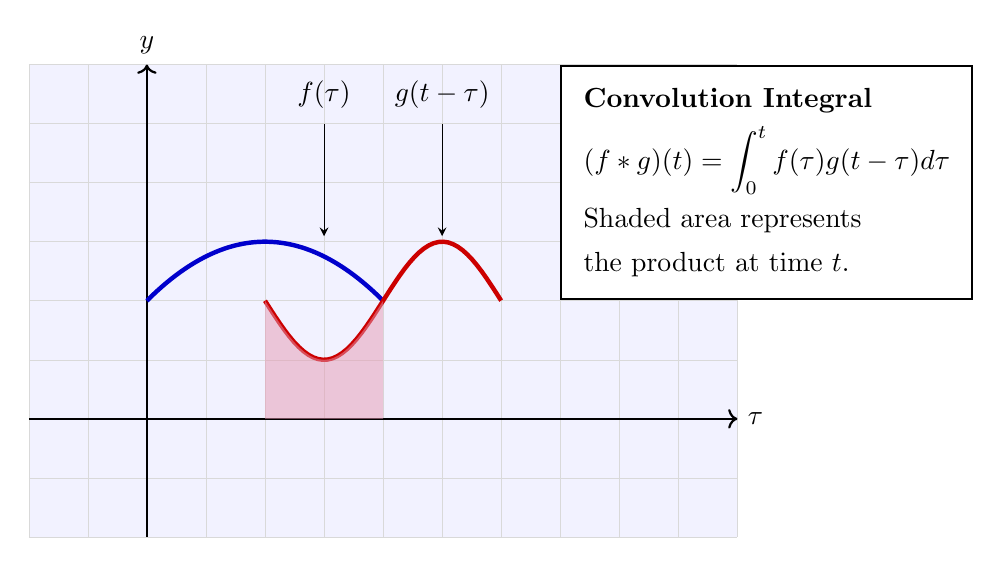
\begin{tikzpicture}[scale=1.5]
    \fill[blue!5] (-1,-1) rectangle (5,3);
    \draw[step=0.5, gray!30, very thin] (-1,-1) grid (5,3);
    \draw[->, thick] (-1,0) -- (5,0) node[right] {$\tau$};
    \draw[->, thick] (0,-1) -- (0,3) node[above] {$y$};
    
    \draw[ultra thick, blue!80!black, domain=0:2, samples=50] plot (\x, {1.5 - 0.5*(\x-1)^2});
    \draw[ultra thick, red!80!black, domain=1:3, samples=50] plot (\x, {1 + 0.5*sin(deg(\x*pi))});
    
    \fill[purple!40, opacity=0.5] (1,0) -- plot[domain=1:2] (\x, {min(1.5 - 0.5*(\x-1)^2, 1 + 0.5*sin(deg(\x*pi)))}) -- (2,0) -- cycle;
    
    \node[align=left, inner sep=8pt, anchor=west, fill=white, draw=black, thick] at (3.5, 2) {
        \textbf{Convolution Integral}\\[4pt]
        $\displaystyle (f*g)(t) = \int_0^t f(\tau)g(t-\tau)d\tau$\\[4pt]
        Shaded area represents\\[4pt]
        the product at time $t$.
    };
    
    \draw[->, >=stealth, shorten >=2pt] (1.5, 2.5) -- (1.5, 1.5);
    \node[above=2pt] at (1.5, 2.5) {$f(\tau)$};
    
    \draw[->, >=stealth, shorten >=2pt] (2.5, 2.5) -- (2.5, 1.5);
    \node[above=2pt] at (2.5, 2.5) {$g(t-\tau)$};
\end{tikzpicture}
\end{center}

\textbf{Tips and Pitfalls:}
\begin{itemize}
    \item \textbf{The $y_k(t)$ Trap:} When solving an IVP using $y(t) = (h * g)(t) + y_k(t)$, students frequently forget to add $y_k(t)$ (the solution to the homogeneous equation with the given initial conditions). Convolution only accounts for the forcing function $g(t)$ assuming zero initial conditions.
    \item \textbf{Variable Confusion:} In the integral $\int_0^t f(t-v)g(v) \, dv$, the integration variable is $v$. Treat $t$ as a constant during the integration.
    \item \textbf{Multiplication vs. Convolution:} Never assume $\mathscr{L}^{-1}\{F(s)G(s)\} = f(t)g(t)$. This is a fatal conceptual error.
\end{itemize}

\newpage
\section{Part 5: Conceptual Synthesis and The "Big Picture"}

\subsection{A) Thematic Connections}
The core theme of convolution is \textbf{superposition in continuous time}. In earlier algebra, if a system's output to an input $x_i$ is $y_i$, the output to $\sum x_i$ is $\sum y_i$. Convolution extends this to continuous functions. We slice the input $g(t)$ into an infinite number of infinitesimally thin impulses. The system's response to each impulse is the impulse response $h(t)$, shifted in time. The convolution integral is simply the continuous sum (superposition) of all these overlapping, shifted impulse responses.

\subsection{B) Forward and Backward Links}
\textbf{Backward Links:} Convolution relies heavily on the foundational calculus concept of the Riemann sum (accumulating area) and the algebraic properties of the Laplace transform (translating differential calculus into algebraic manipulation).
\textbf{Forward Links:} This topic is the absolute bedrock for \textbf{Green's Functions} in Partial Differential Equations (PDEs). In PDEs, the Green's function acts exactly like the impulse response $h(t)$, but in multiple spatial dimensions. Furthermore, in Digital Signal Processing (DSP), continuous convolution is discretized to design finite impulse response (FIR) filters.

\section{Part 6: Abstract Real-World Modeling (AI, ML, \& Quant Finance)}

\subsection{A) Concrete Scenarios}
1. \textbf{Generative AI (Convolutional Neural Networks):} In computer vision, discrete convolution is used to extract features from images. A kernel (filter) slides over the input pixel matrix, computing dot products to detect edges, textures, and shapes.
2. \textbf{Quantitative Finance (Hawkes Processes):} In high-frequency algorithmic trading, the arrival of buy/sell orders is modeled using a self-exciting point process. The intensity of order arrivals depends on the convolution of past events with an exponentially decaying kernel, capturing the "market microstructure" memory.

\subsection{B) Model Problem Setup: Stochastic Volatility and Hawkes Processes}
Let $N(t)$ be a counting process representing the number of market trades up to time $t$. We model the conditional intensity $\lambda(t)$ (the rate of order arrivals) as a Hawkes process:
\[
\lambda(t) = \mu + \int_{-\infty}^t \alpha e^{-\beta(t-s)} \, dN(s)
\]
Here, $\mu > 0$ is the baseline background intensity. The integral is a convolution of the exponential decay kernel $h(t) = \alpha e^{-\beta t}$ with the differential of the counting process $dN(s)$ (which can be viewed as a sum of Dirac delta functions at event times $t_i$). 

If we take the expectation $\E[\lambda(t)] = \Lambda$, and assume stationarity, we can use the Laplace transform of the convolution to find the expected rate of trades. Taking the Laplace transform of the expectation equation yields:
\[
\mathscr{L}\{\Lambda\} = \frac{\mu}{s} + \mathscr{L}\{h(t)\} \mathscr{L}\{\E[dN(t)/dt]\} \implies \frac{\Lambda}{s} = \frac{\mu}{s} + \left(\frac{\alpha}{s+\beta}\right)\frac{\Lambda}{s}
\]
Solving for $\Lambda$ algebraically in the $s$-domain gives $\Lambda = \frac{\mu \beta}{\beta - \alpha}$, which is a fundamental result in market microstructure theory, proving that the system is only stable if $\alpha < \beta$.

\newpage
\section{Part 7: Common Variations and Untested Concepts}

\textbf{Concept 1: Convolution with the Dirac Delta Function}
The homework did not explicitly test the convolution of a function with the Dirac delta function, which is a critical property in signal processing.
\textit{Theorem:} $f(t) * \delta(t-a) = f(t-a)$ for $a \ge 0$.
\textit{Example:} Evaluate $y(t) = \sin(t) * \delta(t-\pi)$.
\textit{Solution:} By the sifting property of the delta function inside the convolution integral:
\[
\int_0^t \sin(t-v)\delta(v-\pi) \, dv = \sin(t-\pi) = -\sin(t) \quad \text{(for } t \ge \pi \text{)}
\]

\textbf{Concept 2: Discrete Convolution}
In modern computing, continuous functions are sampled. The discrete convolution of two sequences $f[n]$ and $g[n]$ is:
\[
(f * g)[n] = \sum_{m=-\infty}^{\infty} f[m]g[n-m]
\]
\textit{Example:} Let $f = [1, 2, 1]$ and $g = [1, -1]$. Find $f * g$.
\textit{Solution:} We slide $g$ across $f$ and compute the dot products:
At $n=0$: $1(1) = 1$.
At $n=1$: $2(1) + 1(-1) = 1$.
At $n=2$: $1(1) + 2(-1) = -1$.
At $n=3$: $1(-1) = -1$.
Result: $[1, 1, -1, -1]$.

\section{Part 8: Advanced Diagnostic Testing: "Find the Flaw"}

\textbf{Problem 1:} Find $\mathscr{L}^{-1}\left\{\frac{1}{s^2(s-2)}\right\}$.
\textit{Flawed Solution:} $\mathscr{L}^{-1}\left\{\frac{1}{s^2}\right\} = t$ and $\mathscr{L}^{-1}\left\{\frac{1}{s-2}\right\} = e^{2t}$. Therefore, the inverse transform is $t e^{2t}$.
\textit{Correction:} The flaw is assuming $\mathscr{L}^{-1}\{F(s)G(s)\} = f(t)g(t)$. The correct approach is convolution: $t * e^{2t} = \int_0^t (t-v)e^{2v} \, dv = \frac{1}{4}e^{2t} - \frac{1}{2}t - \frac{1}{4}$.

\textbf{Problem 2:} Evaluate $e^t * e^t$.
\textit{Flawed Solution:} $e^t * e^t = \int_0^\infty e^{t-v}e^v \, dv = \int_0^\infty e^t \, dv = e^t[v]_0^\infty = \infty$.
\textit{Correction:} The flaw is using the bounds $[0, \infty)$ instead of $[0, t]$ for causal functions. The correct integral is $\int_0^t e^{t-v}e^v \, dv = \int_0^t e^t \, dv = t e^t$.

\textbf{Problem 3:} Solve $y'' + y = \delta(t-\pi), \ y(0)=0, y'(0)=0$.
\textit{Flawed Solution:} $s^2Y + Y = e^{-\pi s} \implies Y = \frac{e^{-\pi s}}{s^2+1}$. Thus $y(t) = \sin(t-\pi) = -\sin t$.
\textit{Correction:} The flaw is forgetting the Heaviside step function $u(t-\pi)$ required by the second shifting theorem. The correct answer is $y(t) = \sin(t-\pi)u(t-\pi) = -\sin(t)u(t-\pi)$.

\textbf{Problem 4:} Find the transfer function for $y'' - 4y' + 4y = g(t)$.
\textit{Flawed Solution:} $s^2Y - 4sY + 4Y = G(s) \implies H(s) = \frac{1}{s^2-4s+4} = \frac{1}{(s-2)^2}$. The impulse response is $h(t) = e^{2t}$.
\textit{Correction:} The flaw is an incorrect inverse Laplace transform for a repeated root. $\mathscr{L}^{-1}\left\{\frac{1}{(s-2)^2}\right\} = t e^{2t}$, not $e^{2t}$.

\textbf{Problem 5:} Simplify $f(t) * (g(t) \cdot h(t))$.
\textit{Flawed Solution:} By the distributive property of convolution, $f(t) * (g(t) \cdot h(t)) = (f(t) * g(t)) \cdot (f(t) * h(t))$.
\textit{Correction:} The flaw is assuming convolution distributes over multiplication. Convolution distributes over \textit{addition}, $f * (g + h) = f*g + f*h$. There is no simple identity for $f * (g \cdot h)$.

\end{document}